\documentclass[10pt]{article}
\usepackage[T1]{fontenc}
\usepackage{lmodern}
\usepackage{amsmath,amssymb,booktabs,graphicx,microtype,tabularx,array,float}
\usepackage[margin=1.7cm]{geometry}
\usepackage{xcolor}
\usepackage[hidelinks]{hyperref}
\definecolor{deepblue}{HTML}{35618F}
\definecolor{warningred}{HTML}{B33A3A}
\newcolumntype{Y}{>{\raggedright\arraybackslash}X}
\newcommand{\C}{\mathbb C}
\newcommand{\R}{\mathbb R}

\title{Fixed-Geometry Looped Attention for the Linear Sampling Method\\
\large Scope correction and experimental status}
\author{}
\date{August 4, 2026}

\begin{document}
\maketitle
\vspace{-2.2em}

\begin{abstract}
This note corrects the scope of the first proof of concept.  The implemented
experiment is one-dimensional Gaussian-process regression from direct point
samples.  It tests a matched fixed softmax/RBF geometry and a tied iterative
kernel solver, but it is \emph{not} an experiment on the Linear Sampling Method
(LSM).  The LSM references instead concern two-dimensional inverse acoustic
scattering, complex multistatic or correlation matrices, and a family of
regularized linear systems indexed by two-dimensional sampling points.  We
state the correct source regimes for the three supplied references, formulate
the appropriate Bayesian least-squares loop, and specify the experiments
required before any result can be described as ``ICL for LSM.''  The existing
1D numbers are retained only as a numerical unit test for the fixed-feature
solver mechanism.
\end{abstract}

\section{Scope correction}

The previous note used ``LSM'' as though it denoted a generic least-squares
model.  In the cited literature it means the \textbf{Linear Sampling Method}
for inverse scattering.  This distinction changes the problem completely.
The current experiment samples
\[
 f\sim\mathcal{GP}(0,k_{\rm RBF}),\qquad
 y_i=f(x_i)+\varepsilon_i,\qquad x_i\in[-1,1],
\]
and reconstructs the scalar function $f$ by kernel ridge regression.  There is
no scattering field, no obstacle, no complex response matrix, and no LSM
indicator.  It is therefore classical 1D GP regression, exactly as the visual
reconstructions suggest.

The correct LSM object is a sound-soft obstacle $D\subset\R^2$.  At a fixed
wavenumber $k$, an incident field $u^i$ generates a radiating scattered field
$u^s$ satisfying
\begin{equation}
 \Delta u^s+k^2u^s=0\quad\text{in }\R^2\setminus\overline D,
 \qquad u^s=-u^i\quad\text{on }\partial D,
 \label{eq:helmholtz}
\end{equation}
together with the Sommerfeld radiation condition.  The inverse problem is to
recover the geometry of $D$ from near- or far-field measurements.

\section{What the Linear Sampling Method solves}

In an active far-field experiment with incident plane-wave directions
$\widehat d_j$ and receiver directions $\widehat x_i$, the data are the
complex multistatic matrix
\begin{equation}
 F_{ij}=u_\infty(\widehat x_i,\widehat d_j),
 \qquad F\in\C^{m\times n}.
 \label{eq:farfield}
\end{equation}
For each probing point $z\in\Omega\subset\R^2$, LSM approximately solves
\begin{equation}
 Fg_z=\phi_z,
 \qquad
 (\phi_z)_i=\frac{e^{i\pi/4}}{\sqrt{8\pi k}}
 e^{-ik\widehat x_i\cdot z},
 \label{eq:lsm-equation}
\end{equation}
using SVD/Tikhonov regularization.  A standard indicator is
\begin{equation}
 I_D(z)=\bigl(\|g_z\|_2^2+\tau\bigr)^{-1/2}.
 \label{eq:indicator}
\end{equation}
The field $z\mapsto I_D(z)$ is evaluated on a \emph{two-dimensional} probing
grid; large values identify the obstacle.  With random illumination, the
matrix $F$ is replaced by a near-field correlation matrix $C$ or a modified
matrix $\widetilde C$, but the sampling equation and indicator logic remain.

\begin{figure}[H]
\centering
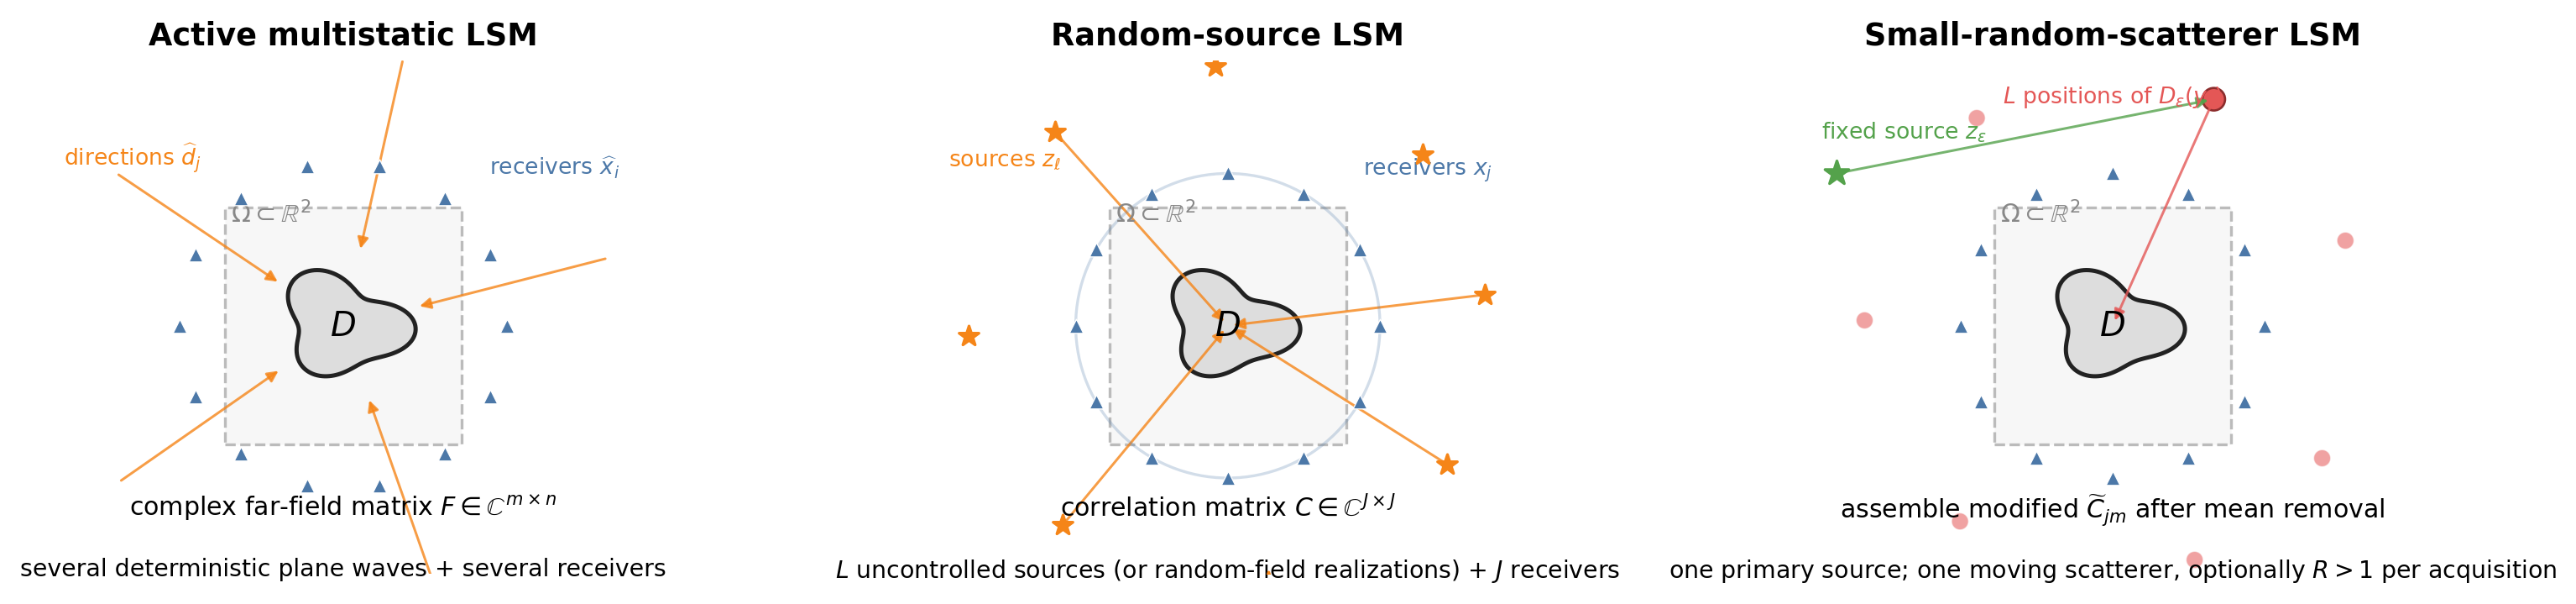
\includegraphics[width=\linewidth]{lsm_reference_geometries.png}
\caption{The three acquisition regimes in the supplied references.  The
random quantity is different in each regime; ``random-source LSM'' should not
be conflated with random GP function samples.}
\label{fig:geometries}
\end{figure}

\section{One or several sources?  Random or deterministic?}

The three papers study different acquisition models.  The following table is
the precise interpretation relevant to a new experiment.

\begin{table}[H]
\centering
\small
\caption{Acquisition regimes in the supplied references.}
\begin{tabularx}{\linewidth}{@{}p{2.15cm}p{1.25cm}YYY@{}}
\toprule
Reference & dimension & illumination/source regime & measured data & reconstruction setting \\
\midrule
Garnier--Haddar--Montanelli (2023)
& theory $d=2,3$; numerics 2D
& Several uncontrolled point sources $z_\ell$ on an enclosing surface; alternatively a continuous random source observed over $M$ realizations.
& Receiver cross-correlation $C\in\C^{J\times J}$, approximating the imaginary near-field matrix.
& Full and limited aperture; base experiment $J=L=80$; $100\times100$ probing grid; ellipse and kite. \\
\addlinespace
Garnier--Haddar--Montanelli (2024)
& 2D
& One fixed, controlled primary point source.  One small scatterer changes random position over $L$ acquisitions and acts as a secondary random source.  An extension uses $R>1$ small scatterers per acquisition.
& Mean-removed measurements form a modified correlation matrix $\widetilde C\in\C^{J\times J}$.
& $J=120$, normally $L=150$ perturbed positions; $L=400$ for i.i.d. positions; one or several target obstacles; $100\times100$ probing grid. \\
\addlinespace
Chenu--Haddar--Montanelli (2026)
& 2D
& Active deterministic full aperture: several plane-wave emitters and several receivers.
& Far-field matrix $F\in\C^{m\times n}$.
& Fixed RBF-DeepONet trunk; single disks in training, noncircular and two-obstacle tests; LSM validates/refines the neural indicator. \\
\bottomrule
\end{tabularx}
\end{table}

Thus the answer is not simply ``one source'' or ``many sources.''  In the 2023
paper there are many random primary sources.  In the 2024 paper there is one
deterministic primary source, while the random moving small scatterer supplies
the diversity; several small scatterers are a separate extension.  In the 2026
paper the acquisition sources are several deterministic plane waves; the
randomness lies in training obstacles and measurement noise, not in the source
configuration.

\section{Our method: fixed nonlinear GP geometry and looped Bayesian LSM}

The references define the physical task; they do not define the proposed
learning method.  Let $A_D$ be the complex, task-dependent LSM matrix:
$F_D^\delta$, $C_D^\delta$, or $\widetilde C_D^\delta$.  The unknown
$g_z$ is indexed by the fixed acquisition nodes $\xi_j$: incident directions
$\widehat d_j$ in the far-field setting, or receiver/source locations $x_j$ in
the correlation setting.  We prescribe a complex GP prior
\begin{equation}
 g_z(\xi)\sim\mathcal{CN}(0,\kappa_\Gamma),\qquad
 (K_\Gamma)_{j\ell}=\kappa_\Gamma(\xi_j,\xi_\ell),
 \label{eq:gp-prior}
\end{equation}
on this acquisition geometry.  The nonlinearity is chosen from the desired
kernel, not learned as a temperature.  On a circular array, for example,
\begin{equation}
 \kappa_\Gamma(\theta,\theta')
 =\exp\!\bigl(\gamma\cos(\theta-\theta')\bigr),\qquad
 S_{j\ell}
 =\operatorname{softmax}_{\ell}
 \bigl(\gamma\cos(\theta_j-\theta_\ell)\bigr),
 \label{eq:periodic-softmax}
\end{equation}
gives a periodic positive kernel and its row-normalized nonlinear attention.
Other Helmholtz- or aperture-adapted kernels may be prescribed in exactly the
same way.

With residual covariance $\Sigma$ and prior covariance
$K_g=\tau^2K_\Gamma$, Bayesian least squares gives
\begin{equation}
 g_z^{\rm post}
 =\arg\min_g
 \|A_Dg-\phi_z\|_{\Sigma^{-1}}^2+\|g\|_{K_g^{-1}}^2
 =K_gA_D^*(A_DK_gA_D^*+\Sigma)^{-1}\phi_z.
 \label{eq:bayesian-lsm}
\end{equation}
The prior scale $\tau$, residual model $\Sigma$, and kernel
$\kappa_\Gamma$ are modelling choices.  They are not outputs of a network.
The tied recurrent attention cell solves the dual system in context:
\begin{align}
 H_D&=A_DK_gA_D^*+\Sigma,\nonumber\\
 q_z^{(t+1)}
 &=q_z^{(t)}
 +\eta_tP_D\bigl(\phi_z-H_Dq_z^{(t)}\bigr)
 +\beta_t\bigl(q_z^{(t)}-q_z^{(t-1)}\bigr),\qquad
 g_z^{(T)}=K_gA_D^*q_z^{(T)}.
 \label{eq:loop}
\end{align}
Only the shared solver dynamics---for example a low-dimensional controller for
$(\eta_t,\beta_t)$ or a structured preconditioner---are trained.  The measured
operator $A_D$, the kernel nonlinearity, and the Bayesian covariance model stay
explicit.

The posterior covariance
\begin{equation}
 \Gamma_D
 =K_g-K_gA_D^*H_D^{-1}A_DK_g
 \label{eq:posterior-covariance}
\end{equation}
quantifies the uncertainty of the regularized inverse and is useful for
acquisition design.  A Bayesian LSM indicator can be defined from the
posterior expected prior norm,
\begin{equation}
 I_D^{\rm Bayes}(z)
 =\left(
 (g_z^{\rm post})^*K_g^{-1}g_z^{\rm post}
 +\operatorname{tr}(K_g^{-1}\Gamma_D)+\tau_0
 \right)^{-1/2}.
 \label{eq:bayesian-indicator}
\end{equation}
For fixed $A_D$, $K_g$, and $\Sigma$, the trace term is independent of $z$:
it calibrates the indicator magnitude but does not create spatial contrast.
The two-dimensional field $z\mapsto I_D^{\rm Bayes}(z)$ may optionally share a
second fixed output kernel
$\kappa_\Omega(z,c)=\exp[-\|z-c\|^2/(2\ell_\Omega^2)]$, with
$z,c\in\Omega\subset\R^2$.  This output geometry is distinct from both the
acquisition kernel $K_\Gamma$ and the task-dependent operator $A_D$.

\paragraph{Explicit distinction from the 2026 method.}
Chenu--Haddar--Montanelli learn a preliminary indicator and a noise estimate,
combine them into a spatial regularization function, and then run classical
LSM.  That is \emph{not} the method proposed here.  We do not train a DeepONet
surrogate of the indicator and do not learn a regularization map.  The loop
itself performs the Bayesian LSM solve from $(A_D,\phi_z)$, while the nonlinear
kernel geometry is fixed by construction.

\section{What the completed 1D experiment establishes---and does not}

The existing experiment remains a useful unit test for matched fixed features
and tied iteration, but its interpretation is deliberately narrow.

\begin{table}[H]
\centering
\caption{Current implementation versus the required LSM experiment.}
\begin{tabularx}{\linewidth}{@{}p{3.2cm}YY@{}}
\toprule
Component & current experiment & correct LSM experiment \\
\midrule
Physical domain & interval $[-1,1]$ & probing domain $\Omega\subset\R^2$ \\
Task & fresh scalar RBF-GP draw & fresh obstacle $D$, source realization, and noise \\
Observation & direct values $f(x_i)+\varepsilon_i$ & complex $F_D^\delta$, $C_D^\delta$, or $\widetilde C_D^\delta$ \\
Linear system & $(K+\lambda I)\alpha=y$ & $(A_DK_gA_D^*+\Sigma)q_z=\phi_z$ \\
Output & reconstructed scalar function & 2D Bayesian LSM indicator from $g_z=K_gA_D^*q_z$ \\
Geometry varied at evaluation & context locations & emitters, receivers, aperture, $L/M$, $k$, and 2D query points \\
\bottomrule
\end{tabularx}
\end{table}

At 12 direct samples, the matched 1D loop reaches MSE $0.1205$, compared with
$0.1136$ for exact KRR, $0.1370$ for a standard Transformer, and $0.2090$ for
the mismatched kernel.  These numbers support the solver unit test only.  They
provide no empirical evidence about obstacle localization, LSM regularization,
random-source cross-correlations, or inverse scattering.

\section{The experiments that must replace it}

The correct proof of concept should proceed in three controlled stages.

\paragraph{Stage A: deterministic active LSM.}
Fix $k=2\pi$, full-aperture source/receiver circles, $m=n\in\{20,30,40,50\}$,
and a 2D probing grid.  Generate complex far-field matrices for random disks,
ellipses and kites.  Train the tied Bayesian loop through the sampling-equation
residual and obstacle-level indicator loss, never by imitating an exact linear
solve and never by learning the kernel or a spatial regularization map.
Evaluate against SVD--Tikhonov--Morozov LSM, with single disks in-distribution
and noncircular or multiple obstacles out-of-distribution.

\paragraph{Stage B: random-source LSM.}
Construct $C_D^\delta$ from receiver cross-correlations.  Sweep the number of
receivers $J$, random sources $L$, source perturbation $\beta$, number of random
field realizations $M$, noise, and aperture.  For i.i.d. random sources or
empirical correlations, the reference theory predicts an
$O(L^{-1/2})$ or $O(M^{-1/2})$ acquisition error; this is a genuine scaling axis
that the learned loop should inherit rather than a context-length law from 1D
GP regression.

\paragraph{Stage C: one source with random small scatterers.}
Fix one controlled primary source, assemble $\widetilde C_D^\delta$ from
$L$ positions of a small scatterer, and then test $R>1$ simultaneous small
scatterers.  The relevant scaling variables are $J$, $L$, $R$, the small
scatterer size $\varepsilon$, noise, aperture, and recurrent depth.

For all stages, report relative indicator error, Dice/IoU, boundary Hausdorff
or Chamfer distance, localization error, contrast, residual norm, and runtime.
Plain latent-function MSE is insufficient.  Experimental design must also
respect controllability: in active acquisition one may choose incident and
receiver directions; in passive random-source acquisition the sources are not
controllable, so the design variables are receiver placement, aperture, and
acquisition duration/number of realizations.

\section{Status}

The present code should be labelled \emph{1D fixed-kernel regression control},
not \emph{LSM}.  No LSM claim is supported until the input is a complex
scattering/correlation matrix and the output is a 2D indicator produced through
the sampling equations above.  The fixed nonlinearity idea remains relevant,
but only as a prescribed 2D feature/prior geometry coupled to the actual
task-dependent LSM operator.

\begin{thebibliography}{9}
\bibitem{randomsources}
J.~Garnier, H.~Haddar, and H.~Montanelli.
\newblock The linear sampling method for random sources.
\newblock \emph{arXiv:2210.15560}, 2023.
\newblock \url{https://arxiv.org/abs/2210.15560}.

\bibitem{randomscatterers}
J.~Garnier, H.~Haddar, and H.~Montanelli.
\newblock The linear sampling method for data generated by small random scatterers.
\newblock \emph{arXiv:2403.19482}, 2024.
\newblock \url{https://arxiv.org/abs/2403.19482}.

\bibitem{neuraloperator}
V.~Chenu, H.~Haddar, and H.~Montanelli.
\newblock A neural operator framework for solving inverse scattering problems.
\newblock \emph{arXiv:2602.24147}, 2026.
\newblock \url{https://arxiv.org/abs/2602.24147}.
\end{thebibliography}

\end{document}
